%\documentclass[11pt,twoside,openany]{is2}
\documentclass[11pt,twoside,openright]{styles/is2}
%%
%% TOGGLE TO MAKE REMARKS VISIBLE
%%
%%\newcommand{\remark}[1]{\begin{quotation}\textit{#1}\end{quotation}}
%%\newcommand{\remark}[1]{}

\usepackage[hyperfootnotes=false, colorlinks=false, pdfborder={0 0 0}]{hyperref}
\usepackage{psfrag}
\usepackage{graphics}
\usepackage{graphicx}
%\usepackage[T1]{fontenc}
%\usepackage[latin1]{inputenc}
\usepackage[english]{babel}

\usepackage{boxedminipage}
\setlength{\fboxsep}{4mm}
\usepackage{todonotes}
\usepackage[inline]{enumitem}
\usepackage{float}
%\usepackage{afterpage}
%\usepackage{subfig}
%\usepackage{theorem}
%\usepackage{tabularx}
%\usepackage{helvet}
%\usepackage{a4wide}
\usepackage{times}
%\usepackage{palatino}
\usepackage{makeidx}
\usepackage{amsmath}
\usepackage{amssymb}
%\usepackage{mathptm}
%\usepackage{moreverb}
%\usepackage{picinpar}
%\usepackage{fancyhdr}
%\usepackage{alltt}
%\usepackage{fancybox}
%\usepackage{eepic}
\usepackage{wrapfig}
\usepackage{epsfig}
%\usepackage{doxygen}
\usepackage{styles/hangcaption}
%\usepackage[dvips]{rotating}
\usepackage{rotating}
\usepackage[hang]{subfigure}
\usepackage{styles/algo}
%\usepackage{textcomp,xspace}
\usepackage{listings}
%For inkscape \usepackage{import}
\usepackage{xifthen}
\usepackage{pdfpages}
%Need for inkscape coloured and transparent images
\usepackage{transparent}
\usepackage{xcolor}
\usepackage{calc}
\graphicspath{{figures/inkscape/}} %Location of pdf files.
%Export object's size than
%documents. %for Tikz standalone package
\usepackage[subpreambles=true]{standalone}
\usepackage{tikz}
\usetikzlibrary{shapes,external}
\usepackage{svg}
\usetikzlibrary{arrows,backgrounds}
\usepgflibrary{shapes.multipart}
%\renewcommand{\sfdefault}{cmss}
%\usepackage{subcaption}
\renewcommand{\floatpagefraction}{0.75}
\sloppy
\setlength{\parskip}{4pt}
\setlength{\parindent}{0pt}
\usepackage{listings}
%\pagestyle{headings}
%\makeindex

\setcounter{tocdepth}{2}
\hyphenation{ana-ly-sis opera-tion opera-tions opera-tio-nal neglected}


\newcommand{\rot}[1]{

\begin{rotate}{-60}

#1

\end{rotate}

}


\newcommand{\upw}[1]{

\begin{rotate}{90}

#1

\end{rotate}

}

\newcommand{\longpage}{\enlargethispage{\baselineskip}}
\newcommand{\shortpage}{\enlargethispage{-\baselineskip}}



% macht durch Kapitelwechsel entstandene leere Seiten auch wirklich leer

% entnommen aus der Doku zum fancyhdr Paket Ver. 1.99d

\makeatletter

\def\cleardoublepage{\clearpage\if@twoside \ifodd\c@page\else

\hbox{}

\vspace*{\fill}

\begin{center}

%This page was intentionally left blank.

\end{center}

\vspace{\fill}

\thispagestyle{empty}

\newpage

\if@twocolumn\hbox{}\newpage\fi\fi\fi}

\makeatother


%%%%%%%%%%%%%%%%%%%%%%%%%%%%%%%%%%%%%%%%%%%%%%%%%%%%%%%%%%%%%%%%%%%%%%%%%%%%%%%
%                        BEGIN OF THE DOCUMENT                                %
%%%%%%%%%%%%%%%%%%%%%%%%%%%%%%%%%%%%%%%%%%%%%%%%%%%%%%%%%%%%%%%%%%%%%%%%%%%%%%%


\begin{document}
% bstctlcite MUST be at the very beginning of your document,
% otherwise, it will "miss" some/most of your cites
\bstctlcite{IEEEtranBST:BSTcontrol}

%\title{FIXME: TITLE OF YOUR THESIS}
%\title{Exploration and Implementation of LEON3\\ SPARC V8 Architecture Using LISA}
\authortitel{cand.-ing.}
\author{Deepak Ramani}
\signature{Deepak Ramani}
\typ{Master Thesis FIXME: ISS-INTERNAL NUMBER}
\betreuer{Shawan Taha Mohammed}
\matnr{314726}
\date{Sep 30, 2020}

\monat{FIXME: CURRENT MONTH}
\maketitleis2

%%% Local Variables: 
%%% mode: latex
%%% TeX-master: "diplomarbeit"
%%% End: 

%\tableofcontents

\newlength\dunder
\settowidth{\dunder}{\_}
\newcommand{\twound}{\rule{2\dunder}{0.4pt}}
\newcommand{\oneund}{\rule{2\dunder}{0.4pt}}

\chapter{Introduction}

The last decade has seen massive growth in the field of Autonomous
Driving, primarily due to 
\begin{enumerate*}[label= \alph*)]
    \item proliferation of graphical processing unit(GPU),

    \item several projects like Google(Waymo) \cite{Waymo},
        Berkeley-DeepDrive \cite{Berkeley-DeepDrive},
        Apollo \cite{Apollo}, have made their datasets open-source making it
        easier for people to work on these data and achieve better performance gains. 
\end{enumerate*}



Training a deep neural network(DNN) forms the core of making a car autonomous. 
By using supervised learning, one can achieve reliable results as it gives greater control
at each stage of training. The data-driven approach collects data in advance and labels it
appropriately. It can then be fed to the DNN using supervised
learning algorithms to train the best model possible. 

Ever since the discovery of Alexnet in 2012 \cite{Alexnet2012}, the convolutional neural network(CNN) and
deep learning(DL) are preferred choices to analyse images.  However, it is well known that the camera sensors are susceptible even to a slight change in weather conditions. 
Sensors like radar \cite{Radar}, LIDAR \cite{LIDAR}, ultrasonic\cite{ultrasonic}, depth camera
give additional depth information for obstacle detection. These values then are fused with the camera images to make
data fusion possible. 

Even though there are some public data available, it is still not enough to reliably
train a DNN. Then there is  the cost of building an autonomous car. Fortunately, the last
years have seen growth in reliable simulators which
helped massively to collect data to help explore this field of research.
To name a few simulators that are being actively used -- LGSVL \cite{LGSVL}, Nvidia Drive
\cite{NvidiaSimulator}, Carla \cite{CarlaSimulator}, CarMaker \cite{CarMaker}. 
In this thesis, the LGSVL simulator is used.

The LGSVL simulator allows the use of different sensors with minimal effort. The data
from different sensors are published through websocket. So to capture these data, we
need an interface/protocol which can understand the sent data's message types and enable the
receiving node/programme to store them. However, the data from each sensor arrives at
different rates. Hence it is necessary to collect and synchronise them in the order of their arrival
before storing, to not lose their integrity and thereby prevent corrupting the dataset.
Robotic operating system(ROS) \cite{ROS2} and its functionalities fulfil
this purpose. It allows seamless transfer of simulator's data by subscribing to it in the
form of topics. Then the subscribing node synchronises it as necessary for storage.

So, now the data that resembles real-world is stored locally for later analysis and
research.

\begin{figure}[h]
    \begin{center}
        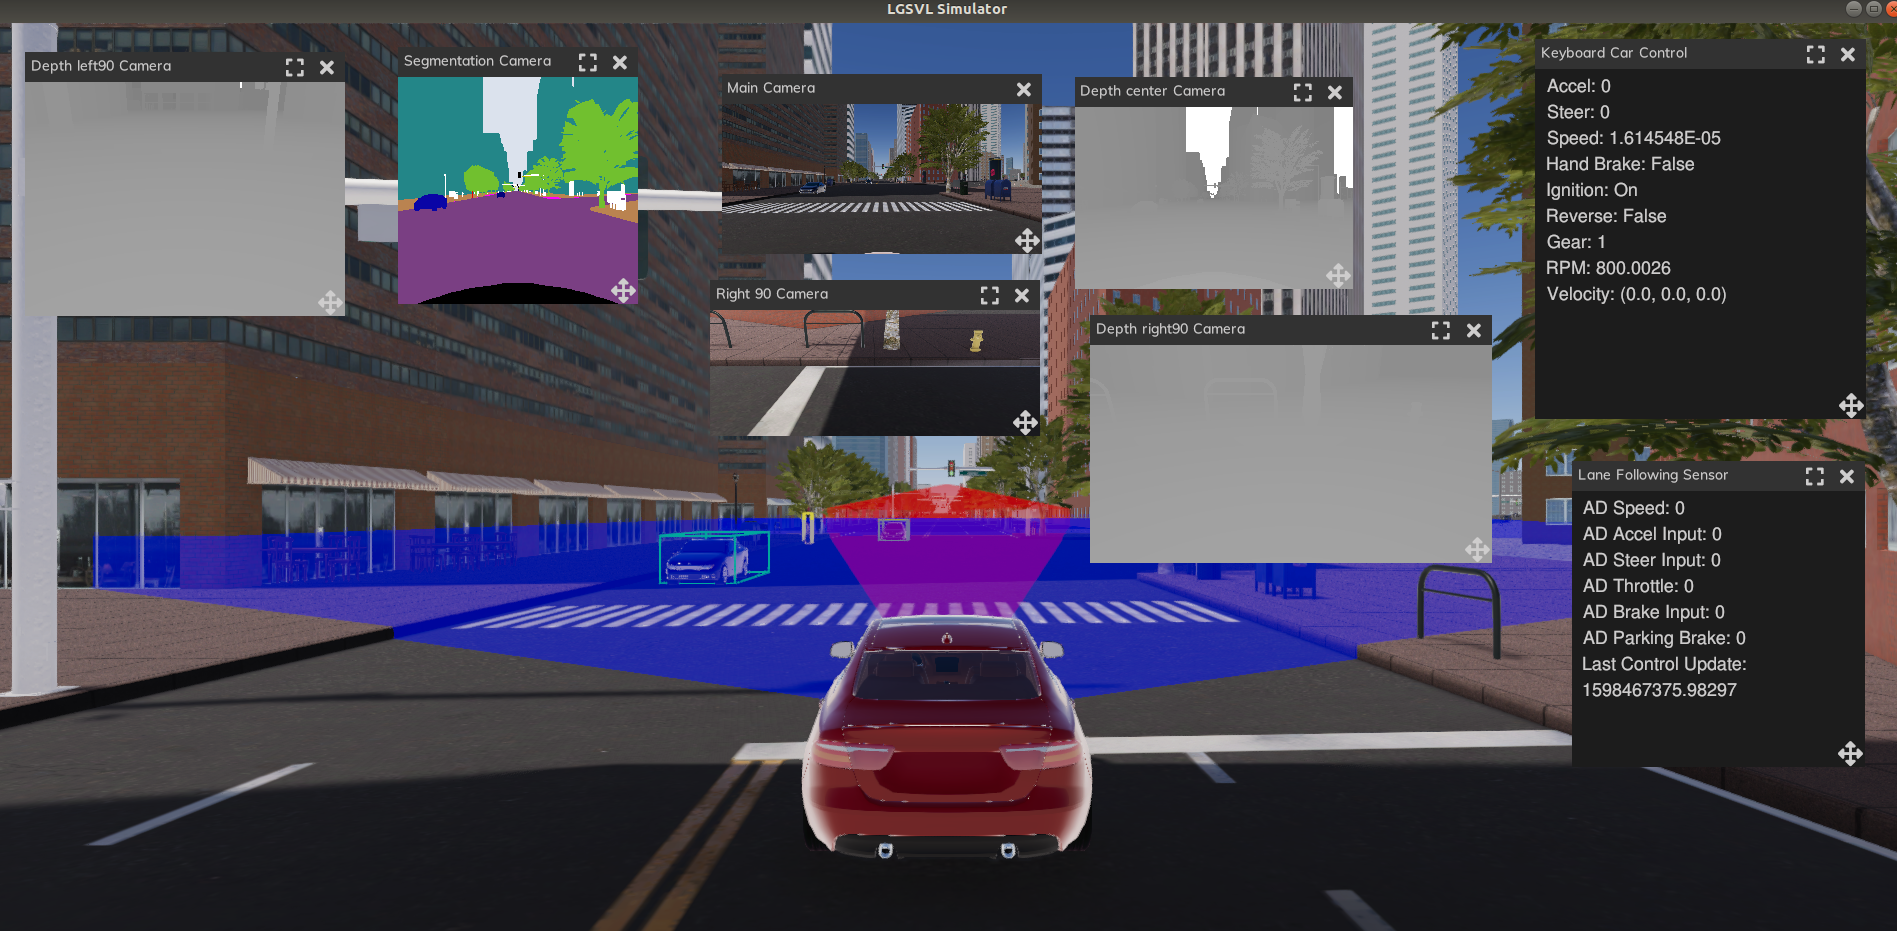
\includegraphics[width = \textwidth]{figures/png/intro/LGSVL_2_scrot_2020-08-26_20-46-55.png}
    \end{center}
    \caption{LGSVL\cite{LGSVL} simulator active with all sensors}
        \label{fig:LGSVL_constellation_sensors}
\end{figure}

\section{Motivation}

Though autonomous driving is one of the favourite research areas in mobility, 
a significant challenge is still the cost associated with integrating all the necessary sensors.  
Representing the environment around the vehicle(ego vehicle) requires information from all in-car sensors. 
The resources demanded to make an optimal decision are also a challenge. The motivation for this thesis is 
to use a simulator, do the required tests and 
determine whether using a simulator does indeed help in perceiving the environment 
and accomplish the goal of driving in the real-world. 

As briefly mentioned, the high cost of associated sensors such as LIDAR
\cite{VergeReportLidar},  has put off many smaller research groups from implementing into their
work. By using a simulator, again at a low cost, we can conduct adequate tests 
on how different constellation of sensors work, how different modalities interact with each other and 
what impact these factors have on the overall performance of the DNN.

Finally, implement an end-to-end system which simulates real-world behaviour which can
then be applied to future research and make it more robust.

\begin{figure}
    \centering
    \def\svgwidth{\columnwidth}
    \input{figures/inkscape/jaguar_sensor_constellation.pdf_tex}
\end{figure}

%%%%%%%%%%%%%%%
%TODO - 
%insert a table 2.1 in page10 showing how different sensor combo work. Use the thesis under
%reference in firefox.
%https://www.researchgate.net/profile/Markus_Weber14/publication/342283221_Autonomous_Driving_Radar_Sensor_Noise_Filtering_and_Multimodal_Sensor_Fusion_for_Object_Detection_with_Artificial_Neural_Networks/links/5eebe41d458515814a6aa417/Autonomous-Driving-Radar-Sensor-Noise-Filtering-and-Multimodal-Sensor-Fusion-for-Object-Detection-with-Artificial-Neural-Networks.pdf 
%%%%%%%%%%%%%%%%

\section{Goal}
    The desired goals of this thesis are listed below: 

\begin{itemize}
    \item Building an autonomous driving framework -
        \begin{itemize}
        \item ROS - use ROS2 to synchronise the data received from the simulator through a
            rosbrige, use functionalities such as slop and cache, to sort the data according to
            their received time in order not to scramble the information. During the evaluation,
            use the same functionalities to send command controls to the simulator.
        \item Rosbridge - use a bridge transport protocol that connects the ros on the receiving end
            to the simulator on the sending end or vice versa.
        \item Docker - set up a work environment that is independent of hardware or
            operating system which allows easy running of the commands for data collection
            and evaluation.
        \end{itemize}    
    \item Implement an end-to-end neural network architecture which learns to drive by
        training from image pixels to steering commands. Also, apply state of
        the art DL techniques to it.
    \item Implement a system that can efficiently collect and label data.
    \item Implement and analyse different constellation of sensors with different data
        fusion techniques. 
\end{itemize}

\section{Related Work}
In 2012, Alexnet \cite{Alexnet2012} used CNNs to do object classification which, then
in Computer Vision became the dominated approach for classification. Both Chen \textit{et
al.} \cite{chen2017} and Bojarski \textit{et al.} \cite{bojarski2016end} extended
\cite{Alexnet2012}'s approach of using CNN and detailed that in addition to classification, CNN can
extract features from images. Then they went on to demonstrate through an end-to-end
network(which self-optimises itself based on its inputs) steering angles can be predicted that keep the car in the
lane of a road. 

In a different field, but using CNN, Sergey Levine \textit{et al.} 
\cite{GooglePaperonCNNActuation} in 2016 corroborated that it was indeed possible to extract
features with CNN and predict motor control actions in \textit{object picking robots}.

Then, Xu \textit{et al.} \cite{XuGYD16CNNLSTM} in the same year with CNN-LSTM architecture
showed that using the previous ego-motion events helped predict future ego-motion events. 
Using CNNs in an end-to-end architecture raised some questions on how it reached its
decisions. So in 2017, both \cite{heatmapsLearning}, \cite{BojarskiCNN1} did visual
analysis after the CNN layers to better understand the module's functionality. 
Vehicle control is more than just steering control. For smoother control, acceleration and
braking are necessary besides steering. Both acceleration and deacceleration are dependent on  the user's driving
style, lane speed limit and traffic etc. Yand \textit{et
al.} \cite{E2EMultimodalDiscreteSpeed} used CNN-LSTM architecture and provided the LSTM
with feedback speed to determine the velocity of the ego vehicle.

Besides vehicle control, perceiving the environment is necessary for collision avoidance. 
The RGB colour camera sensors don't provide the depth information which is critical for collision avoidance. 
Hence, it is essential to fuse other sensors with diverse modalities with RGB to predict an optimal output. 
Liu \textit{et al.} \cite{liu2018learn} provided rules in fusing data. They said that it was
essential to pick out only vital information and discard other noisy data. 
They also described the techniques involved in data fusion -- early/late
fusion, hybrid fusion, model ensemble and joint training. Park \textit{et
al.} \cite{ParkHBB16} gave us methods to enhance the features by using feature amplification
or multiplicative fusion. Zhou \textit{et al.} \cite{ZhouSideChannel} detailed how fusing
data into CNN affects the overall performance.  

Even though the fused dataset gives a performance boost, it performs worse  
compared to individual modality. The combined fused model overfit more
than its counterparts. The fundamental drawback of
\textit{gradient descent} in backpropagation causes the networks to overfit. This paper \cite{wang2020makes} introduced a technique
called \textit{gradient blending} to counteract this problem.

Xiao \textit{et al.}\cite{XiaoCodevillaMultimodalE2E} applied all the fusion techniques
mentioned above with an imitation based end-to-end network\cite{codevilla2017endtoend}. RGB images with depth information(obtained through a different modality)
could indeed result in better performing end-to-end network model was their conclusion.


\section{Contribution}





\chapter{Fundamentals}
\label{chapter:fundamentals}
\section{Machine learning: What and why?}
Machine learning is all about learning from data; gaining knowledge from it. More the
data, more the chances to learn. Machine learning was initially thought of as automating
redundant human tasks and later developed into something that allowed solving complex
mathematical problems. It was seen just an addition to humans than extension of them.
Machine learning these days are required to perform tasks that are quite obvious and
natural to humans such as recognising faces in images or perceive the road environment
around the vehicle and make decisions instinctively.

All these attributes require to extend the field of machine learning.The figure \ref{fig:ai_ml_dl} shows how artificial
intelligence(AI) is divided into specific areas -- Machine learning(ML) and deep learning(DL).

So, in this chapter, a brief overview is given on the concepts that are implemented in the later chapters.

\begin{figure}[h]
	\centering
    \def\svgwidth{0.5\textwidth}
    \input{figures/inkscape/aimldl.pdf_tex} %use full path to know the location of pdftex
    \caption{Schema of AI, ML and DL}
    \label{fig:ai_ml_dl}
\end{figure}

\subsection{Learning algorithms}
Machine learning provides a means to tackle tasks that are complex to solve through fixed
programmes and designed by human beings \cite{Goodfellow-et-al-2016}. A learning algorithm
is an algorithm which gains the ability to learn from data. A ML algorithm is one that
gains the ability to learn from an experience E with respect to some class of tasks T and
performance measure P \cite{mitchell1996m}. With experience, the algorithm can improve its
performance.

\subsubsection*{Tasks, T}
The two major tasks in ML are \textit{classification} and \textit{regression}.

In classification related tasks, the system identifies which of \textit{k} categories an
input belongs to. A function $f : \mathbb{R}^n \rightarrow\{1, \ldots,k\}$ is used by the
learning algorithm to solve this task. When $y = f(x)$, the model assigns an input
described by vector $\mathbf{x}$ to a category
identified by numeric code $y$. There are other variants of the classification
task, for example, where $f$ outputs a probability distribution over classes
\cite{Goodfellow-et-al-2016_1}. Alexnet \cite{Alexnet2012} is one of the examples of
classification task that used it to do object recognition.

Regression is similar to classification except that the output is a continuous value.

A function $f: \mathbb{R}^n \rightarrow \mathbb{R}$ predicts a numerical value for some input.
Predicting the steering control value is a prime example for a regression task.

There are of course other tasks but only classification and regression are used in this
thesis. Hence the narrow focus.

\subsubsection*{Performance measure, P}
To evaluate the performance of a ML algorithm, it is a must to design quantitative measure
of its performance. Usually this performance measure P is specific to a task T. There
are two distinct types of measurements -- accuracy and error rate.

If the goal is to learn a mapping from inputs $x$ to outputs $y$, where $y \in \{1,\ldots
, C\}$, with $C$ being the number of classes. If $C = 2$, this is
called binary classification (in which case we often assume $y \in \{0, 1\})$; if $C > 2$, this is called
multi class classification. If the class labels are not mutually exclusive (e.g., somebody may be
classified as tall and strong), we call it multi-label classification
\cite{murphy2013machine_1}.

Accuracy is a proportion of how much the model produces the correct outputs.
So in the case of binary classification, if the function $f$ predicts a probability
densities $\hat y \in \{0.3, 0.7\}$, for a ground truth $y$ of value $1$, then P is $70\%$
accurate or the error rate is $30\%$.

It is essential that the model is evaluated with a data that it has not seen before. This data
\textit{testing set}, gives a good judgement on the performance  of the trained model.

\subsubsection*{Experience, E}
The ML algorithms can be classified into \textit{supervised}, \textit{unsupervised} and
\textit{reinforcement} learning based on the kind of experience they are allowed to have.
A learning algorithm is allowed to gain experience by going through the \textit{dataset}.
A dataset is collection of all the examples for a given task. For example, to classify
which category a shown image belongs to has collection of images as dataset
\cite{cifar10}. Sometimes datasets are also called as \textit{data points}.

The focus will be on supervised learning in our case.  A random vector $\mathbf{x}$ explicitly attempts to
learn the probability distribution $p(\mathbf{x})$ and predicts $\mathbf{y}$ from
$\mathbf{x}$, usually estimating $p(\mathbf{y}\mid\mathbf{x})$. The CIFAR
dataset \cite{cifar10}, for example, contain images as features which inturn have \textit{targets} or
\textit{labels} associated with it. Here supervised learning(SL), the target
functionality(labels) is known. So it uses the images and predicts the probability
distribution to classify the images in the corresponding label.

\section{Deep Learning}
Deep learning is a subset of machine learning. It takes all the algorithms, concepts from
the machine learning, and narrows the focus to enable a model learn from data such that tasks
involve less human involvement, huge amount of data, and parameters.

\subsection{Simple neural network}
\textit{Linear regression} is one of the common SL algorithms. It solves the regression
problem. For example, if there is vector $\mathbf{x} \in \mathbb{R}^n$ as input and
predict a scalar value $y \in \mathbb{R}$ as its output, then in linear regression, output
is a linear function of the input. We can define it as
\begin{equation}
    \hat y = \mathbf{w}^T\mathbf{x}
    \label{eq:linear equation}
\end{equation}
where $\mathbf{w} \in \mathbb{R}^n$ is a vector of parameters.

$\mathbf{w}$ is usually referred to as a set of weights that determine how each feature
affects the prediction. A $\mathbf{w}_i$ is simply multiplied with a feature $x_i$ to
predict $\hat y$. By manipulating the $\mathbf{w}_i$ value, the corresponding feature $x_i$ has
an effect on the prediction  $\hat y$.

A learning algorithm, in this case linear regression, is implemented as a perceptron. It
is a single-layer neural network as first suggested by Rosenblatt in 1958. They generally consists of four main parts -- input
nodes $x_i$, weights $w_i$, bias $b_0$(if necessary), net sum $\Sigma$ and an activation
function $\sigma$. This is shown in the figure \ref{fig:simpleNN}.

\begin{figure}[h]
    \centering
        \def\svgwidth{0.5\textwidth}
        \documentclass[crop, tikz]{standalone}
\usepackage{tikz}

\usetikzlibrary{positioning}

\tikzstyle{inputNode}=[draw,circle,minimum size=10pt,inner sep=0pt]
\tikzstyle{stateTransition}=[-stealth, thick]

\begin{document}
\begin{tikzpicture}
	\node[draw,circle,minimum size=25pt,inner sep=0pt] (x) at (0,0) {$\Sigma$ $\sigma$};

	\node[inputNode] (x0) at (0, 1.75) {$\tiny +1$};
	\node[inputNode] (x1) at (-2, 0.75) {$\tiny x_1$};
	\node[inputNode] (x2) at (-2, 0) {$\tiny x_2$};
	\node[inputNode] (x3) at (-2, -0.75) {$\tiny x_3$};
	\node[inputNode] (xn) at (-2, -1.75) {$\tiny x_n$};

	\draw[stateTransition] (x0) to[out=-90,in=90] node [midway, right] {$b_0$} (x);
	\draw[stateTransition] (x1) to[out=0,in=150] node [midway, sloped, above] {$w_1$} (x);
	\draw[stateTransition] (x2) to[out=0,in=180] node [midway, sloped, above] {$w_2$} (x);
	\draw[stateTransition] (x3) to[out=0,in=210] node [midway, sloped, above] {$w_3$} (x);
	\draw[stateTransition] (xn) to[out=0,in=240] node [midway, sloped, above] {$w_n$} (x);
	\draw[stateTransition] (x) -- (4.2,0) node [midway,above] {$\sigma\left(w_0 + \sum\limits_{i=1}^{n}{w_ix_i}\right)$};
	\draw[dashed] (0,-0.43) -- (0,0.43);
	\node (dots) at (-2, -1.15) {$\vdots$};
	\node[inputNode, thick] (i1) at (6, 0.75) {$\tiny i_1$};
	\node[inputNode, thick] (i2) at (6, 0) {$\tiny i_2$};
	\node[inputNode, thick] (i3) at (6, -0.75) {$\tiny i_3$};
	
	\node[inputNode, thick] (h1) at (8, 1.5) {$\tiny h_1$};
	\node[inputNode, thick] (h2) at (8, 0.75) {$\tiny h_2$};
	\node[inputNode, thick] (h3) at (8, 0) {$\tiny h_3$};
	\node[inputNode, thick] (h4) at (8, -0.75) {$\tiny h_4$};
	\node[inputNode, thick] (h5) at (8, -1.5) {$\tiny h_5$};
	
	\node[inputNode, thick] (o1) at (10, 0.75) {$\tiny o_1$};
	\node[inputNode, thick] (o2) at (10, -0.75) {$\tiny o_2$};
	
	\draw[stateTransition] (5, 0.75) -- node[above] {$I_1$} (i1);
	\draw[stateTransition] (5, 0) -- node[above] {$I_2$} (i2);
	\draw[stateTransition] (5, -0.75) -- node[above] {$I_3$} (i3);
	
	\draw[stateTransition] (i1) -- (h1);
	\draw[stateTransition] (i1) -- (h2);
	\draw[stateTransition] (i1) -- (h3);
	\draw[stateTransition] (i1) -- (h4);
	\draw[stateTransition] (i1) -- (h5);
	\draw[stateTransition] (i2) -- (h1);
	\draw[stateTransition] (i2) -- (h2);
	\draw[stateTransition] (i2) -- (h3);
	\draw[stateTransition] (i2) -- (h4);
	\draw[stateTransition] (i2) -- (h5);
	\draw[stateTransition] (i3) -- (h1);
	\draw[stateTransition] (i3) -- (h2);
	\draw[stateTransition] (i3) -- (h3);
	\draw[stateTransition] (i3) -- (h4);
	\draw[stateTransition] (i3) -- (h5);
	
	\draw[stateTransition] (h1) -- (o1);
	\draw[stateTransition] (h1) -- (o2);
	\draw[stateTransition] (h2) -- (o1);
	\draw[stateTransition] (h2) -- (o2);
	\draw[stateTransition] (h3) -- (o1);
	\draw[stateTransition] (h3) -- (o2);
	\draw[stateTransition] (h4) -- (o1);
	\draw[stateTransition] (h4) -- (o2);
	\draw[stateTransition] (h5) -- (o1);
	\draw[stateTransition] (h5) -- (o2);
	
	\node[above=of i1, align=center] (l1) {Input \\ layer};
	\node[right=2.3em of l1, align=center] (l2) {Hidden \\ layer};
	\node[right=2.3em of l2, align=center] (l3) {Output \\ layer};
	
	\draw[stateTransition] (o1) -- node[above] {$O_1$} (11, 0.75);
	\draw[stateTransition] (o2) -- node[above] {$O_2$} (11, -0.75);
	
	\path[dashed, double, ultra thick, gray] (x.north) edge[bend left=0] (h5.north);
	\path[dashed, double, ultra thick, gray] (x.south) edge[bend right=0] (h5.south);
\end{tikzpicture}
\end{document}

        \caption{A simple neutral network}
        \label{fig:simpleNN}
\end{figure}

\subsection{Activation function}
\label{subsec:activationfunction}
The common activation functions used are Rectified Linear unit(ReLu), Sigmoid, tanh and
softmax function. For each type of activation, $\sigma$ then decides if the input received is
relevant or not relevant. To convert linear inputs to non-linear, all that has to be done
is to use a non-linear activation function. The figure \ref{fig:activationfunctions},
shows the characteristics of some of the activation functions.

\begin{figure}[h]
	\begin{center}
   \def\svgwidth{0.5\textwidth}
    \input{figures/inkscape/activationfn.pdf_tex} %use full path to know the location of pdftex
	\end{center}
    \caption{Activation functions}
    \label{fig:activationfunctions}
\end{figure}

For classification tasks, usually the last layer of the networks is equipped with softmax
activation layer. This function normalises the output to a probability distribution over
predicted output classes.

\subsection{Multilayer feedforward networks}
\label{subsec:MLP}
Deep feedforward networks or multilayer perceptrons are the quintessential deep learning
models. Its goal is to approximate function $f^*$. In the below figure \ref{fig:MLP},
information flows from inputs $\mathbf{x}$ to output $y$ using a mapping function
$\mathbf{y} = f(\mathbf{x};\mathbf{\theta})$ where $\theta$ are the parameters values
which the MLP learns for optimal approximation.

They are called feedforward as there are no feedback connections in which outputs of the
model are fed back into itself. Feedforwards networks with feedbacks are called
\textit{recurrent neutral networks}.

Feedforwards networks form the core for many commercial applications. For example, the
convolutional neural networks used for object detection are a special kind of feedforward
networks.
\begin{figure}[h]
    \def\svgwidth{0.5\textwidth}
	\begin{center}
        \input{figures/inkscape/inputhiddenoutput.pdf_tex} %use
    \end{center}
    \caption{Multi layer perceptrons}
    \label{fig:MLP}
\end{figure}

More the hidden layers, more the depth of the feedforward networks. The width is given by
the dimensionality of the hidden layer.

\subsection{Loss function}
\label{subsec:lossfunction}
As mentioned before, a mapping function $f$ noisily approximates the input $x$ to output
$y$. So, the noise or the deviation from the true value(ground truth) must be kept at
minimum. The function that calculates the deviation is called \textit{cost} or
\textit{loss} function. It is important to choose the right loss function for a model.

\begin{figure}[h]
	\centering
    \def\svgwidth{0.5\textwidth}
    \input{figures/inkscape/mse.pdf_tex} %use full path to know the location of pdftex
    \caption{Mapping from x to y. The predictor is shown as linear line. The distance
    between the true values and predictor gives the loss. The sum of all the distances
gives the loss function.}
\label{fig:loss function}
\end{figure}

For multi-label classification tasks, \textit{categorical cross-entropy} function is used.
For each category, cross-entropy is calculated. The difference between the cross-entropy
of training data and the model's predictions is the cost function.
\begin{equation}
  CCE = -\frac{1}{N}\sum_{i = 1}^N [\hat{y_{i}}\log(y_{i})  + (1- \hat{y_{i}})\log(1-y_{i})
   \label{eq:CCE}
\end{equation}

For regression tasks, the models are subjected to loss functions such as \textit{mean
absolute error}(MAE), \textit{mean squared error}(MSE) and \textit{mean squared
logarithmic error}(MSLE). In MAE, the mean of absolute differences among predictions and
expected results are calculated.
\begin{equation}
    MAE = \frac{1}{n}\sum_{i=1}^n\left |y_i -\hat y_i \right|
   \label{eq:MAE}
\end{equation}
In MSE, the mean of squared differences among predictions and true outputs are
calculated.
\begin{equation}
    MSE = \frac{1}{n}\sum_{i=1}^n (y_i - \hat y_i)^2
    \label{eq:MSE}
\end{equation}
In MSLE, the mean of relative distances between predictions and true outputs are
calculated.
\begin{equation}
    MSLE = \frac{1}{n}\sum_{i=1}^n(log(y_i+1)-log(\hat y_i+1))^2
    \label{eq:MSLE}
\end{equation}

\subsection{Gradient descent}
\label{subsec:gradientdescent}
Gradient descent is another technique to minimise the cost function parameterised by a
model parameter $\mathbf{w}$. The first derivative(or gradient) gives the slope of the
cost function. Hence, to minimise it, direction opposite to the gradient is chosen.

\begin{figure}[h]
	\centering
    \def\svgwidth{0.5\textwidth}
        \input{figures/inkscape/minima.pdf_tex}
    \caption{Finding the stochastic gradient descent}
    \label{fig:gradientdescent}
\end{figure}

The rate at the which the gradient step reduces is given by the \textit{learning rate}. It
is one of the important parameters in training a model. It is also easily controlled by
the user. If the learning rate is high, greater the step size of each gradient; possibly causing the
step to miss the global minima. Lower the learning rate, more steps or training cycles
needed to reach the global minima. Greater care must be taken in choosing the learning
rate when training a model.

\subsection{Backpropagation}
\label{subsec:backpropagation}
Backpropagation are a class of algorithms which help in training feedforward neural
networks for supervised learning. A model is said to fit when the gradient computation of
the loss function is efficient w.r.t the weights of single input-output in the network.
Backpropagation performs the effective gradient computation using the loss functions
explained above.

\subsection{Optimizer}
\label{subsec:optimizer}
The loss function explains how far the predictions are compared to the true
outputs in a mathematical way. During training process, certain parameters can be tweaked
to help the loss function predict correct and optimised results. However, there are
question such as how to change them, by how much and when?

This is exactly optmizer's function. As explained in \ref{subsec:gradientdescent}, gradient
descent and learning rate form the core of optimizer's functionality. \textit{Stocastic
gradient descent}(SGD) is one of the oldest techniques in which gradients for all of
training examples are calculated on every pass. Hence, they are slow
and require much computation power. Some of the other popular optimizers are Adam
\cite{kingma2014adam}, Adagrad \cite{adagradpaper}, RMSprop \footnote{RMSprop is an unpublished, adaptive learning rate
method proposed by Geoff Hinton in Lecture 6e of his Coursera Class \cite{RMSProp}}. In this work, Adam is used. Adam stands for adaptive moment estimation.
It is a combination of all the advantages of two other extensions of SGD -- Adagrad and
RMSprop. Adam is computationally efficient, straight forward to implement, invariant to
diagonal rescale of the gradients, less effort need to hyperparameters tuning.

\subsection{Challenges in Machine learning algorithms}
\begin{enumerate}
    \item insufficient labelled data
    \item poor quality data and irrelevant features
    \item overfitting/underfitting a model
\end{enumerate}

The first two issues can be solved if the user is careful during data collection and does
preprocessing before feeding the data into the training model. However, if the training or
the test data is too small, the model is subject to underfitting or overfitting. Though
our aim is to reduce the error in the training set, we also need to reduce the error in
the test set. The gap between training and testing error is also important parameter.
Underfitting occurs when the model is not able to obtain sufficiently low error value for
the training set. And if the gap between training and testing error is too large,
overfitting happens. The sweet spot is to stop training the model when the gap between the
two sets is at a minimum value. \label{inside:formodelcheckpoint} Left of the optimal point, the model underfits. Right of
it, the model overfits. The below figure \ref{fig:overfittingunderfitting} shows it very
well. Validation error is the error calculated for the test set.
\begin{figure}[h]
	\centering
    \def\svgwidth{0.75\textwidth}
   \input{figures/inkscape/overfitting.pdf_tex} %use full path to know the location of pdftex
    \caption{Relationship between capacity and error. Inspired from
    \cite{Goodfellow-et-al-2016}}
    \label{fig:overfittingunderfitting}
\end{figure}


\begin{figure}[h]
	\centering
    \def\svgwidth{0.5\textwidth}
   % \begin{Large}
    \documentclass[crop, tikz]{standalone}
\usepackage{tikz}
\usepackage{bm}
\usepackage{relsize}

\usetikzlibrary{positioning}

\begin{document}
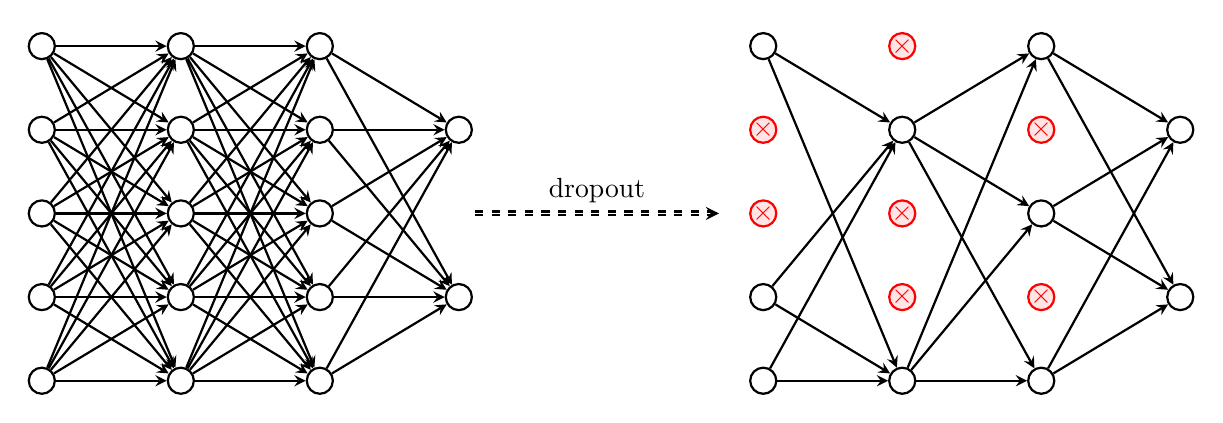
\begin{tikzpicture}

	\node[circle, draw, thick] (i1) {};
	\node[circle, draw, thick, above=2em of i1] (i2) {};
	\node[circle, draw, thick, above=2em of i2] (i3) {};
	\node[circle, draw, thick, below=2em of i1] (i4) {};
	\node[circle, draw, thick, below=2em of i4] (i5) {};
	
	\node[circle, draw, thick, right=4em of i1] (h1) {};
	\node[circle, draw, thick, right=4em of i2] (h2) {};
	\node[circle, draw, thick, right=4em of i3] (h3) {};
	\node[circle, draw, thick, right=4em of i4] (h4) {};
	\node[circle, draw, thick, right=4em of i5] (h5) {};
	
	\node[circle, draw, thick, right=4em of h1] (hh1) {};
	\node[circle, draw, thick, right=4em of h2] (hh2) {};
	\node[circle, draw, thick, right=4em of h3] (hh3) {};
	\node[circle, draw, thick, right=4em of h4] (hh4) {};
	\node[circle, draw, thick, right=4em of h5] (hh5) {};
	
	\node[circle, draw, thick, right=4em of hh2] (o1) {};
	\node[circle, draw, thick, right=4em of hh4] (o2) {};
	
	\draw[-stealth, thick] (i1) -- (h1);
	\draw[-stealth, thick] (i1) -- (h2);
	\draw[-stealth, thick] (i1) -- (h3);
	\draw[-stealth, thick] (i1) -- (h4);
	\draw[-stealth, thick] (i1) -- (h5);
	\draw[-stealth, thick] (i2) -- (h1);
	\draw[-stealth, thick] (i2) -- (h2);
	\draw[-stealth, thick] (i2) -- (h3);
	\draw[-stealth, thick] (i2) -- (h4);
	\draw[-stealth, thick] (i2) -- (h5);
	\draw[-stealth, thick] (i3) -- (h1);
	\draw[-stealth, thick] (i3) -- (h2);
	\draw[-stealth, thick] (i3) -- (h3);
	\draw[-stealth, thick] (i3) -- (h4);
	\draw[-stealth, thick] (i3) -- (h5);
	\draw[-stealth, thick] (i4) -- (h1);
	\draw[-stealth, thick] (i4) -- (h2);
	\draw[-stealth, thick] (i4) -- (h3);
	\draw[-stealth, thick] (i4) -- (h4);
	\draw[-stealth, thick] (i4) -- (h5);
	\draw[-stealth, thick] (i5) -- (h1);
	\draw[-stealth, thick] (i5) -- (h2);
	\draw[-stealth, thick] (i5) -- (h3);
	\draw[-stealth, thick] (i5) -- (h4);
	\draw[-stealth, thick] (i5) -- (h5);
	
	\draw[-stealth, thick] (h1) -- (hh1);
	\draw[-stealth, thick] (h1) -- (hh2);
	\draw[-stealth, thick] (h1) -- (hh3);
	\draw[-stealth, thick] (h1) -- (hh4);
	\draw[-stealth, thick] (h1) -- (hh5);
	\draw[-stealth, thick] (h2) -- (hh1);
	\draw[-stealth, thick] (h2) -- (hh2);
	\draw[-stealth, thick] (h2) -- (hh3);
	\draw[-stealth, thick] (h2) -- (hh4);
	\draw[-stealth, thick] (h2) -- (hh5);
	\draw[-stealth, thick] (h3) -- (hh1);
	\draw[-stealth, thick] (h3) -- (hh2);
	\draw[-stealth, thick] (h3) -- (hh3);
	\draw[-stealth, thick] (h3) -- (hh4);
	\draw[-stealth, thick] (h3) -- (hh5);
	\draw[-stealth, thick] (h4) -- (hh1);
	\draw[-stealth, thick] (h4) -- (hh2);
	\draw[-stealth, thick] (h4) -- (hh3);
	\draw[-stealth, thick] (h4) -- (hh4);
	\draw[-stealth, thick] (h4) -- (hh5);
	\draw[-stealth, thick] (h5) -- (hh1);
	\draw[-stealth, thick] (h5) -- (hh2);
	\draw[-stealth, thick] (h5) -- (hh3);
	\draw[-stealth, thick] (h5) -- (hh4);
	\draw[-stealth, thick] (h5) -- (hh5);
	
	
	\draw[-stealth, thick] (hh1) -- (o1);
	\draw[-stealth, thick] (hh1) -- (o2);
	\draw[-stealth, thick] (hh2) -- (o1);
	\draw[-stealth, thick] (hh2) -- (o2);
	\draw[-stealth, thick] (hh3) -- (o1);
	\draw[-stealth, thick] (hh3) -- (o2);
	\draw[-stealth, thick] (hh4) -- (o1);
	\draw[-stealth, thick] (hh4) -- (o2);
	\draw[-stealth, thick] (hh5) -- (o1);
	\draw[-stealth, thick] (hh5) -- (o2);
	
	\draw[-stealth, double, dashed, thick] (5.5,0) -- node[above] {dropout} (8.6, 0);
	
	
	%%% BOUNDARY %%%
	
	\node[circle, draw, thick, red, fill=red!10, right=15em of hh1] (i1) {};
	\node[circle, draw, thick, red, fill=red!10, above=2em of i1] (i2) {};
	\node[circle, draw, thick, above=2em of i2] (i3) {};
	\node[circle, draw, thick, below=2em of i1] (i4) {};
	\node[circle, draw, thick, below=2em of i4] (i5) {};
	
	\node[red] (icr) at (i1) {$\mathlarger{\mathlarger{\mathlarger{\mathlarger{\mathlarger{\bm{\times}}}}}}$};
	\node[red] (icr) at (i2) {$\mathlarger{\mathlarger{\mathlarger{\mathlarger{\mathlarger{\bm{\times}}}}}}$};
	
	\node[circle, draw, thick, red, fill=red!10, right=4em of i1] (h1) {};
	\node[circle, draw, thick, right=4em of i2] (h2) {};
	\node[circle, draw, thick, red, fill=red!10, right=4em of i3] (h3) {};
	\node[circle, draw, thick, red, fill=red!10, right=4em of i4] (h4) {};
	\node[circle, draw, thick, right=4em of i5] (h5) {};
	
	\node[red] (icr) at (h1) {$\mathlarger{\mathlarger{\mathlarger{\mathlarger{\mathlarger{\bm{\times}}}}}}$};
	\node[red] (icr) at (h3) {$\mathlarger{\mathlarger{\mathlarger{\mathlarger{\mathlarger{\bm{\times}}}}}}$};
	\node[red] (icr) at (h4) {$\mathlarger{\mathlarger{\mathlarger{\mathlarger{\mathlarger{\bm{\times}}}}}}$};
	
	\node[circle, draw, thick, right=4em of h1] (hh1) {};
	\node[circle, draw, thick, red, fill=red!10, right=4em of h2] (hh2) {};
	\node[circle, draw, thick, right=4em of h3] (hh3) {};
	\node[circle, draw, thick, red, fill=red!10, right=4em of h4] (hh4) {};
	\node[circle, draw, thick, right=4em of h5] (hh5) {};
	
	\node[red] (icr) at (hh2) {$\mathlarger{\mathlarger{\mathlarger{\mathlarger{\mathlarger{\bm{\times}}}}}}$};
	\node[red] (icr) at (hh4) {$\mathlarger{\mathlarger{\mathlarger{\mathlarger{\mathlarger{\bm{\times}}}}}}$};
	
	\node[circle, draw, thick, right=4em of hh2] (o1) {};
	\node[circle, draw, thick, right=4em of hh4] (o2) {};
	
	\draw[-stealth, thick] (i3) -- (h2);
	\draw[-stealth, thick] (i3) -- (h5);
	\draw[-stealth, thick] (i4) -- (h2);
	\draw[-stealth, thick] (i4) -- (h5);
	\draw[-stealth, thick] (i5) -- (h2);
	\draw[-stealth, thick] (i5) -- (h5);
	
	\draw[-stealth, thick] (h2) -- (hh1);
	\draw[-stealth, thick] (h2) -- (hh3);
	\draw[-stealth, thick] (h2) -- (hh5);
	\draw[-stealth, thick] (h5) -- (hh1);
	\draw[-stealth, thick] (h5) -- (hh3);
	\draw[-stealth, thick] (h5) -- (hh5);
	
	\draw[-stealth, thick] (hh1) -- (o1);
	\draw[-stealth, thick] (hh1) -- (o2);
	\draw[-stealth, thick] (hh3) -- (o1);
	\draw[-stealth, thick] (hh3) -- (o2);
	\draw[-stealth, thick] (hh5) -- (o1);
	\draw[-stealth, thick] (hh5) -- (o2);

\end{tikzpicture}
\end{document}

    %\end{Large}
    \caption{Illustrating dropout functionality}
    \label{fig:Dropout_function}
\end{figure}

\subsection{Dropout}
DNNs contain multiple non-linear hidden layers and which makes them easily learn
complex relationships between their inputs and outputs. With a small training set, this
relationship adds sampling noise that won't exist in the real-world data even if drawn
from the same distribution. This leads to overfitting and several methods have been
developed to reduce its effect.
\begin{enumerate}
    \item early stopping as soon as the validation error gets worse than the training
        error. \label{item:earlystopping}
    \item L1 and L2 regularisation which penalises the weights \cite{Schmidhuber_2015}.
    \item Randomly drop units(along with their connection) from the neutral network during
        training \cite{dropoutpaper}. Figure \ref{fig:Dropout_function} illustrates how to
        do the random dropping of units.
    \end{enumerate}

\subsection{Convolution Neutral Network - CNN}
Convolutional neural network(CNN) or in short Convnets is a deep learning algorithm for object recognition
tasks. Alexnet \cite{Alexnet2012} was one of the first models to demonstrate the power of
CNNs in object classification. This was then used in various areas of research, where
images were primary inputs, to achieve remarkable extensions. What makes CNN stand out for image
analysis? The network takes images as inputs, reduces them into a form
easier to process, without losing features which are critical for a good prediction. So
not only this is important to consider while designing an architecture but also while
scaling massive dataset.
\subsubsection*{Convolution Layer}
\label{subsubsec:convlayer}
The images which are taken as inputs are just n-dimensional matrix with pixel values. So a
convolution operation can be easily carried on it using a filter or \textit{kernel}. A
kernel matrix is pre-defined according to the task. Usually the size of the kernel is tiny compared to images' which facilitates easy
convolution. A \textit{stride} is the value of a step taken by the kernel after each
convolution. If stride = 1, then it is called \textit{non-strided}. Convolution remarkably
extracts the high-level features such as edges. Normally there are many Convnets in an
architecture. Each layer extracts a different feature or expands on last layer's task.

If the dimensionality of the convolved feature stays the same or increased compared to the
input, then it is called \textit{same padding}. If the dimensionality is reduced,
\textit{valid padding}. Padding is extremely useful for solving boundary conditions.

\subsubsection*{Pooling Layer}
\label{subsubsec:pooling}
This layer is similar to convolutional layer. Its task is to decrease the computational
power required to process data, usually done through reducing the dimensionality. It is,
furthermore, useful to extract dominant features that are rotational and positional
invariant, thus maintaining the goal of training the model.

There are two types of pooling -- \textit{max pooling} and \textit{average pooling}. Max Pooling
returns the maximum value from the portion of the image covered by the Kernel.
On the other hand, Average Pooling returns the average of all the values
from the portion of the image covered by the Kernel. Pooling also helps in reducing the
noisy pixels which sometimes skew feature extraction.

\subsubsection*{Flatten and Fully Connected Layer}
The main goal for extracting features from the images is to do some task; for example -
classification. So the extracted features must be converted into a form understandable for
the MLP (\ref{subsec:MLP}), which happens to be 1-dimensional vector. This is exactly the
task of \textit{flatten layer}.

MLP gets a vector as input and feeds it to a feedforward network in \textit{fully
connected layer}. Fully connected layer then outputs the necessary values depending on the
task.

It is important to remember that each layer employs an activation function(
\ref{subsec:activationfunction}) to introduce linearity or non-linearity to the inputs.

\subsection{Recurrent neural networks - RNN}
One of the drawbacks of neural networks is that they always start from scratch;with no
memory of the previous state. If a neural network has to be used for word prediction,
knowledge of previous letter and word is necessary. Recurrent neural networks addresses
this issue.

RNN provide the temporal dynamic behaviour. A typical RNN looks like in the figure
\ref{fig:RNN}. The left hand side shows it folded and right hand side unfolded in time.
\begin{figure}[h]
	\centering
        \def\svgwidth{0.7\textwidth}
\begin{tiny}
        \input{figures/inkscape/simplernn.pdf_tex}
\end{tiny}
    \caption{A Simple RNN}
    \label{fig:RNN}
\end{figure}
RNN, however, suffers from \textit{long term dependencies}. This is well explored in
\cite{RNNdrawback1} and \cite{RNNdrawback2}.

\subsection{LSTM}
\label{subsubsec:lstm}
The shortcomings of RNN are overcome by LSTM - \textit{Long Short Term Memory}.
They are a special kind of RNN which was first introduced by \cite{LSTMPaper}. They remember
information for long periods as their default behaviour with ease. The figure
\ref{fig:lstm} shows how the structure of a LSTM differs from simple RNN. The LSTM employs
gates and activation functions to add or delete information from the previous state.

\begin{figure}[h]
	\begin{center}
	   \def\svgwidth{0.7\columnwidth}
    \input{figures/inkscape/lstm.pdf_tex} %use full path to know the location of pdftex
	\end{center}
    \caption{LSTM Architecture}
    \label{fig:lstm}
\end{figure}


\section{Sensors}
Deep neural networks need data -- images or measurements to perform necessary tasks. These
information/data are captured using sensors.
\subsection{Visual Sensors}
Visual sensors are one of the commonly used sensors for image capture of the environment.
Usually cameras are used.
\subsubsection*{RGB Colour Camera}
A camera in Red-Green-Blue colour spectrum is used to capture images. These images are
then processed into different spectrum range to do feature analysis.
\subsubsection*{Depth Camera}
A Depth camera returns an image where the shades on the grey-scale correspond to the depth of objects.
\subsubsection*{Segmentation Camera}
This sensor returns an image where objects are coloured corresponding to user-defined tag.
For example, a car is blue, pedestrian red, road boundaries white etc.
\subsection{Measurement Sensors}
These sensors are required for provided information other than visual such as telemetry
data.
\subsubsection*{Radar Sensor}
A common sensor in weather forecast which is known for its long range ability and
resistant to adverse weather conditions. With radar, relative information of the
environment are collected such as distance between vehicles, relative positions of them
etc.
\subsubsection*{Control Sensor}
With this sensor, telemetry information can be collected.

\section{Sensor/Data Fusion}
To allow DNNs make the best perception of the environment, it is necessary to fuse data from
several sensors and feed that combined data into the DNN. This technique of fusing
information exists for decades \cite{Datafusion1}. Often used data fusion technique is
\textit{Kalman filtering} and its variants. Some of the notable papers using that
technique are  \cite{Datafusion3}, \cite{Datafusion2}.

For autonomous driving, RGB and depth information(RGB-D) is vital for obstacle avoidance.
\cite{XiaoCodevillaMultimodalE2E} uses data fusion to get better results for their
experiment.
\subsection{Types of Data Fusion}
There are two traditional approaches to data fusion -- \textit{early fusion} and
\textit{late fusion}.
In early fusion, all the sensor inputs are concatenated before being fed to the CNN.
Whereas in late fusion, each sensor inputs are fed to separate convolutional layer and
down the line, they are concatenated together.

These techniques can be seen in action in this \cite{wang2020makes} recently
published paper from Facebook research team.
\begin{figure}[h]
	\begin{center}
        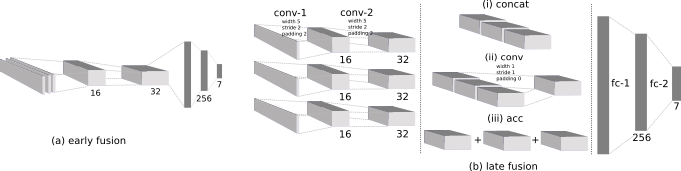
\includegraphics[width=0.8\textwidth]{figures/inkscape/datafusion.png} %use full path to know the location of pd flex
	\end{center}
    \caption{This figure is taken from this \cite{Datafusion4} paper where they describe early and
        late fusion architectures and also present three types of late fusion.}
    \label{fig:Datafusiontypes}
\end{figure}


\section{Machine Learning Library}
To train the neural networks, we need a ML library framework to programme it. \textit{Tensorflow}
\cite{tensorflow},
\textit{Keras} \cite{Keras}, \textit{Pytorch} \cite{pyTorch} are some of the popular ML
frameworks used today.
For this thesis, we use Keras, a python high-level wrapper for tensorflow. With keras, one
can easily design DNN architectures with minimal effort. All the DL techniques we
discussed above are reduced to a bunch of human understandable commands.
Keras has several application programming interfaces(APIs) -- Models, Layers and
Callbacks.
\subsection{Models API}
They are of two types -- Sequential and Functional. Sequential is just stack of layers
with one input and one output. Functional can handle models with non-linear topology,
shared layers, and multiple inputs or outputs. Since functional API offers flexibility, it
is used here.
In addition to offering the overall functionality, this API has the power to implement
optimizers (\ref{subsec:optimizer}), loss functions (\ref{subsec:lossfunction}).

\subsection{Layers API}
The layers needed for CNN -- convolution (\ref{subsubsec:convlayer}), pooling
(\ref{subsubsec:pooling}), normalization, regularization,
activation (\ref{subsec:activationfunction}) and time series operations with LSTMs
(\ref{subsubsec:lstm}) are easily implemented with this API.

\subsection{Callbacks API}
With this API, some of the overfitting challenges can be automatically avoided.
Some functionalities available are early stopping (\ref{item:earlystopping}) and
ModelCheckpoint (\ref{inside:formodelcheckpoint}).

Early stopping sets an epoch parameter \textit{n}. If the gap between training and validation loss
don't improve/reduce for the next \textit{n} defined epochs, the training is automatically
stopped.

With ModelCheckpoint, the gap is monitored w.r.t a monitoring parameter;usually minimum validation
loss or maximum validation accuracy. Then automatically the best model gets saved.

In order to visualise the performance of the training, \textit{TensorBoard} class is used.

\section{Robotic Operating System - ROS}
The Robotic Operating System(ROS) \cite{aboutros} is a set of software libraries and tools created to help
developers build robot applications. From drivers to state-of-the-art algorithms, and with powerful developer tools, ROS is a necessary set of tools for any robotics project. And it’s all open source.

ROS environment was first developed by Willow Garage for the PR2 robot \cite{firstros}. PR2 is a humanoid robot that can navigate autonomously in a known environment.
Since then, ROS is now used in all kinds of robots in various fields. With its popularity,
many companies manufacture ROS compatible robots. This massively helps integrating
multiple components to communicate with each other.

ROS(ROS1), since its launch, was considered as a middleware/interface between components. There was a
parent to which all the children were connected. Every child node had to go through the
parent every time to discover another node.  In today's, expanding robotics market,
this approach is outdated. This led to the development of ROS2 \cite{whyros2}.
\subsection{ROS2}
ROS2 uses a data distribution service(DDS) for publishing and subscribing instead of
custom message handler. With DDS, the transmission performance is also improved. Each node
is \textit{peer-to-peer} and can contact other nodes efficiently.
ROS2 is simply not an extension of ROS1; although some of the functionalities have been
ported.


\subsection{ROS2 concepts}
In this section we will study different concepts used in the thesis.
\subsubsection*{Nodes}
A node is an entity that uses ROS protocol to communicate with each other. In a ROS graph,
there are networks of nodes and connections between them.
\subsubsection*{Messages}
Messages are ROS data type that are used when subscribing or publishing to a topic.
\subsubsection*{Topics}
A topic is named information \textit{bus} over which nodes exchange messages.
A topic usually begins with \textit{"/"} followed by the topic name. For example, "/radar"
is topic associated with radar bus. Each topic carries information of a particular message
type. This message type can either be a standard or custom type.
\subsubsection*{Subscriber and Publisher}
If a node subscribes to a topic, then the node is called a \textit{subscriber}. If it
publishes to a topic, then it is a \textit{publisher}.

Both publisher and subscriber when they are initialised over a topic, a \textit{queue
size} is defined. Depending on the queue size, a topic's messages can be queued and
processed as needed. The figure \ref{fig:rosgraph} shows a subscriber and publisher node
exchange data with each other.

\begin{figure}[h]
    \centering
    \def\svgwidth{0.9\textwidth}
    \input{figures/inkscape/rosgraph.pdf_tex}
    \caption{A graph showing how a publisher or subscriber node interact and exchange
    messages with each other through a topic.}
    \label{fig:rosgraph}
\end{figure}

\subsubsection*{Spins and Callbacks}
In computer programming, spinning is a technique in which a process repeatedly checks to
see if the condition is true. In ROS, a node is set to spin with no or a condition. This
enables it to do its tasks as programmed.

Also from computer programming, callbacks is a function that executes at a given time.
There are two types of callbacks -- \textit{blocking} and \textit{deferred}. In ROS,
deferred callback is used. It means that the callback function is invoked after a node
returns something. It can be a subscriber receiving a message from its subscribed topic.

\subsubsection*{Rosbridge}
We are aware that there are some non-ROS robots which would need to communicate with ROS
ones. So a rosbridge \cite{rosbridge} acts as communication API between these two. The rosbridge
specification is programming language and transport agnostic.

\subsubsection*{Message Filters}
Since the main goal of this thesis is to do data fusion, we need to use ROS to communicate
with different sensor nodes. These sensor nodes receive and transmit data at different rates.
So we need a filter that can trap the received or transmitted messages, serialize them(so
as to not lose data's integrity) and make it possible for storage.

With the help of a filter, all the nodes can be made to wait till every node receives the message and then
invoke the callback function only once or multiple times as per design. Inside the callback, further operations can be
carried out before saving.

\textit{Message\_filter} \cite{messagefilters} is one such filter. It has the
functionalities we are looking for, such as TimeSynchronizer, cache(a buffer to store
messages while waiting for others), and slop(an extra delay parameter to TimeSynchronizer
modules which defines the delay(seconds) with which the incoming messages can be
synchronized.) Caution must be kept when choosing the slop value. Otherwise, the data will
lose its integrity.

In the next chapter, we will see how the LGSVL \cite{rong2020lgsvl} simulator is used.

\section{Docker}
Docker \cite{dockergettingstarted} is an open-source tool designed to make it easier to create, deploy, and run applications by
using containers. These software containers allow developers to package an application
with all the parts it needs, such as libraries and other dependencies, and deploy it as
image based packages. By doing so, developers can be sure that their application will run smoothly
irrespective of the client's environment. This also allows for easy debugging and
development.

Docker can also loosely considered as virtual machine(VM). But unlike a VM, rather than
using a whole operating system, a docker shares the kernel of the system and shipping only
the applications that are not in the host machine. Also a docker container is independent
of host machine's applications. This greatly improves performance.

However, docker has its drawbacks. For example, building a docker image takes sometimes
long to compile and consume a lot of resources. So not everyone can build an image and
regularly as they wish.

In this thesis, docker containers are used for data collection from the simulator and later
for evaluation of the model with the simulator.

\section{Notes:}
\begin{enumerate}
    \item draw cnn
    \item if possible draw for fusion techniques.
\end{enumerate}





\chapter{Simulation and Simulator}
From the beginning of autonomous driving research, simulators have played a key role in
development and testing new algorithms. Simulators allow developers to quickly test their
algorithms without driving real vehicles. In this chapter, we will the conditions a
simulator must satisfy, and go in detail about LGSVL simulator and its development.
\section{Need for a simulator}
One of the important questions to ask before explaining about simulation is to understand
why should one need a simulator to do simulation. As explained in the previous chapter
(\ref{chapter:fundamentals}), deep neural network(DNN) using supervised learning algorithm
needs huge amount of labelled data. Since the cost of collecting that amount of data in
real road vehicle is too expensive, researchers have sought the help of simulators. A
simulator is an application which simulates a real-world environment, virtually. With the
help of a simulator, one can collect any amount of data they wish for their project.

\section{Conditions for a simulator}

Data collection is one of the most important phases in supervised learning. So caution must
be taken in choosing a simulator. A simulator must fulfil certain conditions to be
qualified as a good one.
\begin{itemize}
    \item It must have a vehicle that can move around in a virtual map.
    \item The vehicle must be equipped with appropriate sensors for perceiving the
        environment properly.
    \item The virtual map must try to mirror the real-world to an extent. That mean it
        should have proper terrain to drive around, lane marking for lane detection, other
        cars to mirror the real world traffic, pedestrians, and real world weather
        conditions.
    \item It must provide a medium to collect data and allow interfaces to transfer the
        data. It should also be able to receive data in case the user needs to validate
        the data collected.
    \item Finally and most importantly, support end-to-end, full stack simulation.
\end{itemize}

\section{LG SVL simulator}
A simulator chosen for this thesis is from LG research centre in Silicon Valley,
California called LGSVL simulator. It is an open source project where the code is
regularly published at Github \cite{lgsvlgithub}. This simulator satisfies all the
conditions listed above. They provide an out-of-the-box solution which can meet the
needs of developers wishing to focus on testing their autonomous vehicle algorithms. It
also supports Apollo \cite{ApolloAuto} and Autoware \cite{autowarePaper}.

\subsection{LGSVL simulator development}
LGSVL simulator's core simulation engine is developed using the Unity game engine
\cite{unitygameengine}. Unity game engine is written in C\# programming language. Since a
game engine inherently supports animation, the simulator is able to extend that
functionality easily. In addition to Unity, also supports several libraries necessary to
compute complex mathematical operations. With Unity's latest High Definition Render
Pipeline(HDRP), LGSVL is able to simulate photo-realistic virtual environments that match
the real world.

\subsection{Overview of LG SVL simulator}

\subsubsection*{User AD Stack}
It supports user autonomous driving(AD) stack. That means a user can develop, test and verify through simulation.
The user AD stack connects to LGSVL Simulator through a communication bridge interface; a bridge is selected based
on the user AD stack’s runtime framework. This bridge interface can use a standard
protocol such ROS, ROS2 or custom one like CyberRT \cite{ApolloAuto}.

In addition LGSVL supports plug-in component which a user can develop and attach it to the
simulator. The simulator during runtime picks up this plug-in.

\subsubsection*{Simulation Engine}
As mentioned above, LGSVL uses Unity's latest HDRP game engine.

\subsubsection*{Sensor and vehicle models}
It supports sensor arrangement and importantly they are customisable. The sensors are
added and removed through JSON formatted text along with its parameters. These parameters
include sensor type, position of the sensor, topic name, publishing rate, and in some
sensors reference frame of measurement. Some of the popular sensors like camera sensors,
radar and LIDAR are supported. In addition, users can add their own custom sensors as
plug-in. Fig.\ref{fig:sensortypeslgsvl} gives a good overview of some of the sensors in action.

Vehicles provide a medium to travel the environment. Hence, vehicle dynamics is also
important.

\begin{figure}[!ht]
    \centering
    \def\svgwidth{0.9\columnwidth}
    \input{figures/inkscape/sensordistribution.pdf_tex}
    \caption{Different types of sensors in LGSVL simulator. Anticlockwise(from top): RGB
    colour camera, Segmentation camera, Radar(also 3D bounding boxes), LiDAR, Depth camera}
    \label{fig:sensortypeslgsvl}
\end{figure}

\begin{figure}[!ht]
    \centering
    \def\svgwidth{0.9\columnwidth}
    \input{figures/inkscape/lgsvlsensor1.pdf_tex}
    \caption{Different types of sensors in LGSVL simulator. Anticlockwise(from top): RGB
    colour camera, Segmentation camera, Radar(also 3D bounding boxes), LiDAR, Depth camera}
    \label{fig:sensortypeslgsvlnew}
\end{figure}

\subsubsection*{Environment and maps}
An environment, in this case, virtual, is a primary component in autonomous driving
simulation to provide many input to AD system. An environment affects almost all the
functionalities in a AD system such as perception, prediction and tracking modules. It
also affects the vehicle dynamics which is the key factor in vehicle control mechanism.
Through changes in the HD map, the environment affects localization and planning modules.
Finally, weather conditions such as rain, fog, night driving naturally affect the
environment. So caution must be taken while design the environment.

LGSVL supports creating, editing and exporting HD maps of existing 3d virtual environment.
3D environment also defines the rules about how agents must behave such as stopping at traffic
lights, giving way to priority traffic, respect lane boundaries etc.

As of writing, LGSVL supports virtual Sanfranciso city HD map. They also support smaller
maps like Shalun and Cubetown.

\begin{figure}[h]
    \centering
    \def\svgwidth{\textwidth}
    \input{figures/inkscape/weather.pdf_tex}
    \caption{LGSVL simulator in different weather conditions}
    \label{fig:weatherconditions1}
\end{figure}

\begin{figure}[h]
    \centering
    \def\svgwidth{\textwidth}
    \input{figures/inkscape/lgsvlweatherconditions.pdf_tex}
    \caption{LGSVL simulator in different weather conditions}
    \label{fig:weatherconditions}
\end{figure}

\subsubsection*{Test scenarios}
Test scenarios enable users to test their AD stack by simulating in an environment and
comparing and contrasting correct and expected behaviours. A lot of variables like HD maps,
traffic movement behaviour and their density, time of the day, weather conditions etc. also
play a role while testing. It is also possible to write scripts with the help of Python
API where scenarios can be created and tested.

Thus LGSVL simulator \cite{rong2020lgsvl} provides the best virtual environment to conduct our experiments for
autonomous driving.

\chapter{Implementation}
\label{chapter:implementation}
This chapter will present the implementation of end-to-end network with its extensions.
First we start with docker to set the environment. Then move on to LGSVL and ROS.
From there a closed loop is achieved to collect data, preprocess, introduce neural
network, implement the models, and evaluate it. After achieving the basic results for the
preliminary architecture, sensor fusion techniques are implemented.

\section{Docker}
Docker is an open-source platform for developing, shipping and running applications.
Because docker makes installing applications hardware independent, we use docker for our
tasks.
\begin{wrapfigure}{l}{0.5\textwidth}
	\centering
    \def\svgwidth{0.5\textwidth}
    \input{figures/inkscape/scrot_dockerengine.pdf_tex} %use full path to know the location of pdftex
    \caption{Docker Engine and its functions}
    \label{fig:dockerengine}
\end{wrapfigure}


\begin{figure}[t]
	\centering
    \def\svgwidth{\textwidth}
    \input{figures/inkscape/docker_1.pdf_tex} %use full path to know the location of pdftex
    \caption{Docker and its various functions}
    \label{fig:docker1}
\end{figure}

A docker architecture, as shown in \ref{fig:dockerarchitecure}, consists of client, host
and registry. To make all these components work, docker daemon is necessary. A daemon is a
type of long-running background process. The LGSVL docker image is pulled from the registry using
\textit{docker pull} command. An image is a read-only template with instructions for
creating a docker container. The instructions are provided using a \textit{dockerfile}.
One can then build the images by themselves or use an image that is already built. In our
case since the image is readily available, so we use it.

A docker container for each task can be defined. Along with a task, certain other
services may need to be run along with it. \textit{Docker compose} gives a perfect
solution to manage docker applications.  When setting the environment with docker is difficult in some cases, an anaconda
environment \cite{anacondaenv} is used.

\section{LGSVL simulator}
The LGSVL simulator is developed using Unity engine which is written in C\# language.
The LGSVL team organises their code base\cite{lgsvlgithub} in such a way that it makes it
easy for a beginner to learn the structure and implement new features or change the
existing ones.
\subsection{Web user interface and JSON sensor parameters}
The LGSVL team has developed a web UI to help users to configure maps, vehicles and
simulations. They also support different maps and vehicles configurations.
\begin{wrapfigure}{l}{0.7\textwidth}
	\centering
    \def\svgwidth{0.7\textwidth}
    \input{figures/inkscape/LGSVLsoftwarearchi.pdf_tex} %use full path to know the location of pdftex
    \caption{LGSVL software architecture}
    \label{fig:lgsvlswarchitecture}
\end{wrapfigure}
A sensor configuration is defined in JSON format. If a user wishes to use a colour camera
sensor, then they need to use the JSON format appropriate for this sensor to the vehicle
configuration. Each sensor has a topic name which is then used by ROS nodes to subscribe
to it. In our case, we use a variety of sensors -- RGB colour camera, depth camera,
segmentation camera(output of a RGB camera fed to a neural network), and Radar sensor.
These sensors can be arranged/aligned in different constellations according to
requirements.

So, we have

\begin{enumerate}

    \item a RGB camera placed facing ahead parallel to the ground, another on
the left and right side of the car pointed an angle towards the ground,
    \item a depth camera following same configuration as RGB,
    \item a segmentation camera placed adjacent to the RGB front facing camera,
    \item a radar sensor placed front of the car near to the hood pointing ahead.
\end{enumerate}

The file associated with each sensor then picks up the values from JSON parameters and adjusts it in
run-time. If a sensor functionality is available, a user can use appropriate JSON to
utilise that sensor.

\subsection{Sensor plugin - Data collection and evaluation}
When a user doesn't want to disturb the current setup of the simulator but rather wants to add
some custom sensor to the vehicle configuration, then sensor plugin provides a perfect
solution. A set of guidelines must be followed while developing the plugin. In our case,
it is necessary to have a sensor plugin that would create a sensor and topics. This sensor
and these topics would then be used to fetch data from the simulator, transfer it through ROS bridge, and also receive
data for evaluation of the trained model. This custom plugin
extends the unity engine libraries to read the values from the JSON definition, fetch
values of steering, acceleration, braking from the vehicle control system, do
data transfer between simulator and ROS. The data transfer involves converting data types
to ROS understandable formats and convert back ROS to simulator formats during evaluation
phase.

\subsection{Radar Sensor}
Since data fusion is one of the goals of the thesis, using a radar sensor would provide
important depth information. However, in LGSVL, in its current version, the radar sensor is not working as
required. This necessitates some changes to some of the files in the LGSVL code base.
This process involves -
\begin{enumerate}
    \item Correcting the already existing radar sensor code to detect traffic properly and
        assign the data to their variables that look similar to ROS custom message standards.
    \item Converting the LGSVL data to ROS understandable  custom message formats.
    \item Adding ROS2 as the bridge type to establish between client and LGSVL.
    \item On the client side, editing the docker to include custom radar message types.
\end{enumerate}

LGSVL simulator is now configured to send data towards the client. In order to reach the
client, as mentioned before, a ROS bridge is needed. In the next section we will talk
about ROS and its uses.

\section{Data collection}
For data collection, \textit{python} programming language is used to create scripts. Each
script uses ROS components.

\begin{figure}
	\centering
    \def\svgwidth{\textwidth}
    \input{figures/inkscape/datacollection.pdf_tex} %use full path to know the location of pdftex
    \caption{Data collection module}
    \label{fig:datacollectionmodule}
\end{figure}

\subsection{ROS}
ROS, in our case, acts as an interface between simulator(server) and scripts(client).
We use ROS 2 and in particular \textit{dashing} iteration. The LGSVL follows the ROS standard for the message types.
The ROS nodes listen to the sensor topic(defined using JSON sensor parameter) and invoke
a callback whenever they receive data. Since each sensor receives at different rates, a
filter called message filters is used. With message filters, the queue size is set to a
higher value say 1000 and a delay(in seconds) through a \textit{slop} parameter of value
0.1 is used. This filter gathers all the subscribing nodes as one, synchronises
approximately to the delay parameter and invokes just one callback. This assures that data
from each listening node is present.

Inside the callback, the data is processed using computer vision(CV) and numpy libraries.
The ROS messages for the images include header and data
parts. The header part consists of the time at which the message is created and data part
contains the real data. With numpy libraries the real data is extracted easily for storage.

\subsection{ROS web bridge}
A ROS web bridge is a virtual bridge between scripts using ROS and LGSVL simulator. In this
case, a ROS 2 web bridge, written in nodejs, is established. It basically starts an instance
that listens to an IP address and its port. The LGSVL on the other side, listens to this
IP address and port. Hence a bridge is created to allow flow of data.
\begin{figure}[h]
	\centering
    \def\svgwidth{\textwidth}
    \input{figures/inkscape/ros2bridge.pdf_tex} %use full path to know the location of pdftex
    \caption{ROS2 web bridge implementation}
    \label{fig:ros2webbridge}
\end{figure}
\iffalse
\subsection{Building ROS2 package}
Before running the scripts with ROS, it must be built as ROS packages.  A package is a
container for ROS 2 code which makes it easier to share with others. Package creation in
ROS 2 uses \textit{ament} as its build system and \textit{colcon} as its build tool.
Packages can be created either in \textit{CMake} or \textit{Python}.

For CMake, \texttt{package.xml} and \texttt{CMakeLists.txt} files are necessary. \texttt{package.xml}
file contains meta information about the package. \texttt{CMakeLists.txt} file describes how to build the code within the package.

For Python, \texttt{setup.py}, \texttt{package.xml}, \texttt{setup.cfg} and
\texttt{resource/<package-name>} are needed. The \texttt{package.xml} file contains meta
information about the package. Unlike CMake, \texttt{setup.py} contains instructions on
how to install the package. The \texttt{setup.cfg} is required when a package has
executables, so \textit{ros2 run} can find them. Lastly there is
\texttt{resource/<package-name>}. It is a directory with the same name as the package,
used by ROS 2 tools to find the package. Inside the directory there is \texttt{\twound{init}\twound{.py}}.

In our case, LGSVL team provides the base package. So we need to just build it using
\texttt{colcon build --symlink-install} command. But before building, the ROS2 environment
 must be set. It is important to remember that the package has
to be built every time a new ROS or custom message data types are introduced. \texttt{build},
\texttt{install} and \texttt{log} directories are created along side \texttt{src}
directory when the build command is executed at the parent workspace directory. And
every time before running the package, its local environment must be set. Otherwise,
custom message data types won't be initialised.

\subsection{Using docker-compose services}
So everything that involves ROS starts with setting the environment globally or locally.
It is easy to miss this small step and encounter problems that could take a long time to
resolve. A \texttt{docker-compose} helps alleviate this problem. A service for each task
is implemented such as build, collect and evaluate. In the yaml file, each service has a
keyword to invoke the service and also an argument to link a file. In this case, a
shell script file is created. It contains all the necessary steps
such as setting the environment, starting the package, establishing ROS web bridge etc.
\fi

\begin{figure}
	\centering
    \def\svgwidth{0.6\textwidth}
    \input{figures/inkscape/preprocessing.pdf_tex} %use full path to know the location of pdftex
    \caption{Preprocessing module}
    \label{fig:preprocessing}
\end{figure}

\newpage
\section{Preprocessing}
The stored data can't be always used directly for training. Most times it must be
preprocessed to user's needs and goals.
Inputs are usually represented as \texttt{X\_{data}} and outputs as \texttt{Y\_{data}}. In our case, the input is images and output control commands.
Since we are doing supervised learning, we are aware about the outputs. These are stored in
\textit{csv} files along with file names of the images.

So, the first task in preprocessing is to select which \texttt{Y\oneund{data}} is necessary for prediction
and seperate them out into a small text file. Using this file, the images are fetched,
manipulated using CV2 libraries, stored in arrays and saved in the form of HDF5 files
\cite{hdf5file}. The Hierarchical Data Format version 5 (HDF5), is an open source file format
that supports large, complex, heterogeneous data. Within one HDF5 file, you can store a similar set of data organized in the same way that you might organize files and folders on your computer.
It is a compressed format and supports \textit{data slicing} which allows only a part of
the dataset to be read and not load all of them in the RAM memory.

The images in our case are read either as grayscale or RGB colour images. Then are cropped
and resized to a smaller resolution such as 160x70. For grayscale image there is one
channel. So the image's dimensions resemble 160x70x1 and for RGB image it has 3 channels
which means the dimensions are 160x70x3.

The images from multiple viewpoints or sensors can be fused together making
multi-channels. This task will be explained more in data fusion
section(\ref{sec:datafusion1}).

\subsection{LSTM}


LSTM comprises of serially lined up LSTM cells which allow prediction using previous
data. Since previous data require data from past, each frame image must be backtracked to
a certain, defined time period. This is called \textit{time steps}. According to the time
step, the images(frames) are gathered as one and stored. So for a $time\_step = 15$, the
dimensions will look like \texttt{15x70x160x1} for grayscale images and \texttt{15x70x160x3} for RGB
images.
\begin{figure}[h]
	\centering
    \def\svgwidth{0.8\textwidth}
    \input{figures/inkscape/slidingwindow.pdf_tex} %use full path to know the location of pdftex
    \caption{Sliding frame window implementation module}
    \label{fig:slidingwindow}
\end{figure}

\section{Datafusion}
\label{sec:datafusion1}
Data fusion is one of the primary goals of this thesis. As discussed in fundamentals
chapter(\ref{sec:datafusion}), there are two techniques for data fusion -- early and late
fusion. For early fusion, the images from multiple viewpoints or sensors are fused in the
preprocessing stage. This fusion is accomplished either by stacking the images or
concatenating them. So for example, if a grayscale and RGB images are fused/overlayed together using
concatenation, then the dimensions would like \texttt{70x160x4} where 4 represents number
of channels. These images are usually referred to as \textit{multispectral images}. The figure \ref{fig:cnnarchitecture} illustrates this approach.

Late fusion on the other hand is done during the training stage of the end-to-end work
flow. Usual process involves combining(concatenating) two sources of information after one
or two layers of convolution and then using the combined block to do further feature
extraction and eventually prediction. Or if the source is of a different modality than an
image, then it is unnecessary to fuse them in convolution stage. It is added after
the CNN is completed. However, it must be remembered that late fusion increases the
trainable parameters and costs on resources. The figure \ref{fig:latefusion} illustrates
one of the late fusion processes.

\begin{figure}[h]
    \centering
    \def\svgwidth{\textwidth}
    \input{figures/inkscape/latefusion1.pdf_tex}
    \caption{Late Fusion}
    \label{fig:latefusion}
\end{figure}

\section{Training the model}
\begin{wrapfigure}{l}{0.4\textwidth}
	\centering
    \def\svgwidth{0.4\textwidth}
    \input{figures/inkscape/splitdata.pdf_tex} %use full path to know the location of pdftex
    \caption{Splitting the dataset into train and test data using Sci-kit learn module.}
    \label{fig:splitdata}
\end{wrapfigure}
Training a model involves designing a neural network architecture and deciding on its
hyperparameters. In this thesis, CNN and dense layers are designed with appropriate
activation functions, learning rate, epochs, batch size, CNN specific stride and kernel
lengths, optimizer etc.

\subsection{Loading from HDF5 and splitting the data}
The data stored in HDF5 files in preprocessing are loaded into memory as X\_data and
Y\_data respectively. Then using scikit-learn module, the X\_data is then split 80-20
as X\_train and X\_test respectively. Similarly Y\_data as Y\_train and Y\_test respectively.

\subsection{CNN and fully connected layers}
For CNN layers, feature maps starting from 24 channels is chosen and gradually increased till 64.
The stride is always kept at 2 whereas the kernel size is (5,5) for the early and
(3,3) for the later stages. For early data fusion, the input is already fused and directly
fed to the neural network. However, for late fusion, concatenation is done at appropriate
stages. If necessary, max pooling and batch normalization layers are added to the neural
network. Most often to distribute the features uniformly and to make the cost function
distribute symmetrically, the inputs are normalized. In this case, since images are pixel
values between 0-255, each pixel is divided by 255 to bring it in the range between 0 and
1.
\begin{figure}
    \centering
        \def\svgwidth{1.05\textwidth}
        \input{figures/inkscape/trainingImplementation.pdf_tex} %use full path to know the location of pdftex
    \caption{Implementation of Training module.}
    \label{fig:trainingmodule}
\end{figure}

Since Keras is used, almost all the layers can be implemented in a fewer lines of code.
Activation functions are given as an argument to a layer. Adding new layers is easier with
functional API \ref{subsec:modelsapi}. When the convolutional layers' output needs to be
flattened to form a vector, \texttt{Flatten} command is called.

The fully connected or dense layers take input as a vector. The hyperparameters are
adjusted accordingly to avoid overfitting. Using dropout layers and batch normalization
help alleviate this problem.

Using callbacks functionality of Keras, the best model is saved in HDF5 file. In our case, validation
loss  reaching the minimum is monitored. Since the datasets are not huge, an epoch of 100
is sufficient.

\section{Evaluation}
The trained model is saved as HDF5 file format. Evaluation is basically completes the loop
of end-to-end training architecture. The trained model is placed at a location the
evaluation script can access. Then from the LGSVL simulator data are received through ROS
bridge and subscriber nodes. With the help of message filters, the messages are collected.
Inside the callback, the image manipulation carried out in preprocessing phase, is
repeated. The preprocessed image is then fed to the trained model. The model predicts the
output which in our case, is control commands. These commands are then assigned and published/sent
back to the simulator through ROS bridge. The custom plugin has a subscribing topic on the
LGSVL side. The data sent through ROS bridge, is picked up by nodes listening in this topic. The predicted command behaviour is observed and
evaluated using appropriate metrics. It is important to remember that, the exact steps followed
in preprocessing must be repeated while evaluating. Otherwise, it will lead to inconsistent
performance.

\begin{figure}
	\centering
    \def\svgwidth{\textwidth}
    \input{figures/inkscape/evaluation.pdf_tex} %use full path to know the location of pdftex
    \caption{Evaluation implementation}
    \label{fig:evaluationfigure}
\end{figure}

\iffalse
\section{What to include here?}

\begin{enumerate}
    \item Docker - Dockerfile contents - docker scripts - how they are invoked.
    \item LGSVL - C\# language, Unity engine, code organisation, sensor plugin and its
        structure, data type conversion, WebUI - JSON- sensors used. Making Radar work,
        Increasing traffic density and time at the signal.
    \item Data collection - ROS2- ros2 message types - topics - msgfilters -
        approx-sync - callback- cv2 libraries - saving. Also ROS2 web bridge.
    \item Preprocessing - CV2 image manipulation - stacking, concatenate  -
        Time series LSTM stuff - saving in HDF5.
    \item Training - Loading hdf5 - splitting data - Functional API - normalisation
        - datafusion - early, late - concat - batch normalisation - stride - kernel -
        flatten - FC - prediction - Activation function - loss function - learning rate -
        optimizer - epochs - shuffling - batch size - callbacks - ES - MC - TB - saving
        models.
    \item Evaluation - similar stuff to data collect - image manipulation - prediction -
        publishing. How to validate evaluation?

\end{enumerate}

\fi

\chapter{Evaluation}
In this chapter, the workflow explained in last chapter is evaluated and results are
presented.

Before showing the evaluation, it is necessary to define training and testing conditions
that can be easily used by others to verify the results.

Each evaluation has a setup and its corresponding result.

We have three datasets that can be used for training and evaluation.
\begin{enumerate}
    \item Dataset 1 - Contains 100,000 raw data. It is collected in no traffic
        environment, doing straight driving without any sudden turning. The data is using
        San Francisco map and driven during afternoon. This dataset has only data
        representing centre camera pointed ahead, parallel to the ground and right camera
        pointed to the ground at an angle $20^{\circ}$. The control commands include
        acceleration, throttle, braking, and steering angle values.
    \item Dataset 2 - Also contains 100,000 raw data. It is, however, collect with traffic
        where the cars stop at signal intersections for a longer time than dataset 3. This
        dataset is also collect in San Francisco map and during afternoon. It contains a
        centre camera, right camera like dataset 1, left camera similar to right camera by
        pointing at an angle $20^{\circ}$ to the ground, depth camera sensors placed at
        centre, left and right just like RGB cameras. The control commands are same as
        dataset 1.
    \item Dataset 3 - Contains 270,000 raw data. It is collected while driving around San
        Francisco. About 200,000 data is collected while driving in the afternoon. About
        20,000 in different weather and light conditions. About 50,000 entries are
        collected in a different circular circuit map called CubeTown. In addition to RGB
        and depth cameras distributed just as dataset 2, a segmentation camera is kept
        next centre RGB camera facing forward, and a radar sensor just in front of the
        car near the hood also facing forward.

\end{enumerate}
\section{Evaluation setup}
While evaluating, a testing parameter \textit{episode} is used. Each episode lasts 30 seconds. A timer is started for 30 seconds and
the  model is tested for collisions. If a collision happens, the time at which collision
happened is noted.

\subsection{Setup 1 - Determine the best lighting conditions to test the model}
\label{chapter05subsec:setup1}
All three datasets are used. The test is conducted in San Franciso map without traffic
option switched ON. By varying the light conditions to morning, afternoon and evening, we
observe how light influences the prediction of output. Only steering angle is predicted
and a steady velocity of 3 meter per second is used. An episode length of 30s is used.
When a collision is observed, the time of collision and the count are noted down.
\begin{table}[t]
    \centering
\begin{tabular}{|c c c c|}
    \hline
    time(in 24 hrs standard) & Morning & Afternoon & Evening \\\hline
      & 7:35 & 15:30 & 18:30 \\\hline
\end{tabular}
\end{table}

\begin{figure}
	\centering
    \def\svgwidth{0.6\textwidth}
    \input{figures/inkscape/datasetsLCCollisions.pdf_tex} %use full path to know the location of pdftex
    \caption{Datasets vs Light Conditions vs Number of Collisions}
    \label{fig:dsvslcvsncolsetup1}
\end{figure}

It is seen from figure \ref{fig:dsvslcvsncolsetup1} that afternoon time provides the best light conditions for all the three
datasets. Dataset 1 and 3 perform equally across the three lighting conditions.

If the percentage of number of collisions, as shown in figure
\ref{fig:dsvslcvstrafficavgncolsetup1a}, is calculated, dataset 3 performs the best among
the datasets for morning and afternoon part of the day.
\begin{figure}
	\centering
    \def\svgwidth{0.6\textwidth}
    \input{figures/inkscape/averagecollisionsSetup1.pdf_tex} %use full path to know the location of pdftex
    \caption{Datasets vs Afternoon vs Traffic vs Average number of Collisions}
    \label{fig:dsvslcvstrafficavgncolsetup1a}
\end{figure}

\subsection{Setup 2 - How the datasets perform during afternoon if traffic is enabled?}
All three datasets are again used. The time is fixed at 15:30. The traffic is toggled ON.

\begin{figure}
	\centering
    \def\svgwidth{0.6\textwidth}
    \input{figures/inkscape/Afternoonwithtraffic.pdf_tex} %use full path to know the location of pdftex
    \caption{Datasets vs Afternoon vs Traffic vs Number of Collisions}
    \label{fig:dsvslcvstrafficncolsetup2}
\end{figure}
From figure \ref{fig:dsvslcvstrafficncolsetup2}, we can observe that all three datasets do
well even in traffic. However, it is surprising to see dataset 1 which had no traffic
while the dataset was collected, performs remarkably well when driven in traffic.



\iffalse
-----------------------------

\textbf{Dataset 1} - 100k raw data with no traffic. Just driving straight. First one with just steering and no other training.  With 1 centre camera.

\textbf{Dataset 2} - 100k raw data with traffic and increased wait times at junctions.

\textbf{Dataset 3} - 270K raw data with normal waiting times, increased brake scenario, different weather and light conditions, also driving in different map. With segmentation and radar.

----------------------------

\subsection{Test scenario 1}

----------------

\textbf{Epsiodes} - One minute. Manually start timer and run the evaluation. Count the \# of collisions. If collided, reset episode and start again. If no collision, restart after episode duration(1 min).


\subsection{Test Scenario 2}

---------------

Loss function as constant and using dataset 3. Explain why dataset 3 is being chosen.

CNN architecture should be same!

\textbf{MSE} - output(accel, brake and steering all regression)

\textbf{CCE} - input images(center and center depth). Output(Accel, brake and steering mse)

\textbf{With no traffic} -

Drive for 1 hour and see how model responds.

\textbf{With traffic} -

drive for 1 hour and see how model responds.

Epoch training - 50
\section{Testbed setup}

\begin{enumerate}
    \item dataset constant - Only dry day data?
        or everything?
    \item CNN parameters variable.
    \item epochs, learning rate, optimizer, loss function constant
    \item activation function constant or variable?
    \item for LSTM - timesteps value?
    \item graph - training, val loss vs epochs?
    \item graph - loss vs learning rate?
    \item graph - timesteps vs loss?
    \item graph - evaluation performance comparison?
    \item graph - Accel, brake, noaction predicted vs ?
    \item graph - brake, steering predicted vs ?
    \item graph - accel, brake, steering predicted vs ?
    \item graph - accel,brake, steering, distance(radar) predicted vs ?
    \item graph - with seg camera vs without?
    \item graph - with radar vs without?
    \item graph - imbalanced vs balanced Cross entropy?


\end{enumerate}
\fi

%\include{chapter06_}
%\include{chapter07_}

\begin{appendix}

\listoffigures
%\listoftables
%\listoflistings

\raggedright
\bibliographystyle{IEEEtran}
\bibliography{IEEEabrv,bib/IEEEtranBST,bib/mybib.bib}

\end{appendix}

\end{document}


%%%%%%%%%%%%%%%%%%%%%%%%%%%%%%%%%%%%%%%%%%%%%%%%%%%%%%%%%%%%%%%%%%%%%%%%%%%%%%%
%                          END OF THE DOCUMENT                                %
%%%%%%%%%%%%%%%%%%%%%%%%%%%%%%%%%%%%%%%%%%%%%%%%%%%%%%%%%%%%%%%%%%%%%%%%%%%%%%%
